\documentclass[20pt,landscape,a4paper,footrule]{foils}
\usepackage{solido-network-slides}

\begin{document}
\selectlanguage{english}
\mytitlepage{IPv6 introduction}


\vskip 2cm
\centerline{\footnotesize Slides are available as PDF}

\slide{Goal}
\hlkimage{5cm}{kame-noanime-small.png}

\begin{list1}
\item Introduce IPv6 
\item IPv6 addressing 
\item Neighbor Discovery Protocol
\item IPv4 vs IPv6 - Differences and similarities
\item Practical examples
\item Ressources
\end{list1}

%\centerline{Participate and demonstrate IPv6 working - make the turtle dance!}

\slide{Internet idag}

\hlkimage{14cm}{images/server-client.pdf}

\begin{list1}
\item Clients and servers
\item Rooted in academic networks
\item Protocols which are more than 20 years old
\item Very little encryption and security built into the network
\end{list1}

\slide{Internet is built on Open Standards}
{\hlkbig 
We reject kings, presidents, and voting.\\
We believe in rough consensus and running code.\\
-- The IETF credo Dave Clark, 1992.}

\begin{list1}
\item RFC - Request for comments
\item RFC, Best Current Practice, FYI, informational\\
\item Standards track:\\
Proposed Standard $\rightarrow$ Draft Standard $\rightarrow$ Standard
\end{list1}



%%%%%%%%%%%%%%%%%%%%%%%%%%%%%%%%%%%%%%%%%%%%%%%%%%%%%%%%%%%%%%%%%%%%%%%
%% Node 1: UCLA (30 August, hooked up 2 September) 
%% Node 2: Stanford Research Institute (SRI) (1 October) 
%% Node 3: University of California Santa Barbara (UCSB) (1 November) 
%% Node 4: University of Utah (December) 
%% RFC 4: Network Timetable
%% http://www.zakon.org/robert/internet/timeline/

\slide{Internetworking: history}

\begin{list2}  
\item[1961]  L. Kleinrock, MIT packet-switching theory
\item[1962]  J. C. R. Licklider, MIT - notes 
\item[1964]  Paul Baran: On Distributed Communications
\item[1969]  ARPANET 4 nodes
\item[1971]  14 nodes
\item[1973]  Design of Internet Protocols started
\item[1973]  Email is about 75\% of all ARPANET traffic
\item[1974]  TCP/IP: Cerf/Kahn: A protocol for Packet
        Network Interconnection
\item[1983]  EUUG $\rightarrow$ DKUUG/DIKU forbindelse
\item[1988]  About 60.000 systems on the internet - 
        The Morris Worm hits about 10\%
\item[2002]  Ialt ca. 130 millioner p� Internet
\item[2010] IANA reserved blocks 7\% (Maj 2010) - \link{http://www.potaroo.net/tools/ipv4/}
\end{list2}

\slide{Why IPv6}

\hlkimage{20cm}{ipv4-report.png}

\centerline{\link{http://www.potaroo.net/tools/ipv4/}}

No more talk, we need IPv6, get to work - end of discussion

\slide{OSI \& Internet Protocols}

\hlkimage{14cm,angle=90}{images/compare-osi-ip.pdf}

\slide{IPv6: Internet redesigned? - no!}
 
\begin{list1}
\item Preserve the good stuff
\item back to basics, internet as it used to be!
\item fate sharing - connection rely on end points, not intermediary NAT boxes
\item end-to-end transparency - you have an address and I have an address
\item Wants: bandwidth +10G, low latency/predictable latency, Quality of Service, Security
\end{list1}

\vskip 5mm
\centerline{\color{titlecolor}\LARGE \bf IPv6 is evolution, not revolution}
\vskip 5mm

Note: IPv6 was not designed to solve all problems, so don't expect it to!


\slide{The Internet has done this before!}


\begin{quote}
   Because all hosts can not be converted to TCP simultaneously, and
   some will implement only IP/TCP, it will be necessary to provide
   temporarily for communication between NCP-only hosts and TCP-only
   hosts.  To do this certain hosts which implement both NCP and IP/TCP
   will be designated as relay hosts.  These relay hosts will support
   Telnet, FTP, and Mail services on both NCP and TCP.  These relay
   services will be provided  beginning in November 1981, and will be
   fully in place in January 1982.

  
   Initially there will be many NCP-only hosts and a few TCP-only hosts,
   and the load on the relay hosts will be relatively light.  As time
   goes by, and the conversion progresses, there will be more TCP
   capable hosts, and fewer NCP-only hosts, plus new TCP-only hosts.
   But, presumably most hosts that are now NCP-only will implement
   IP/TCP in addition to their NCP and become "dual protocol" hosts.
   So, while the load on the relay hosts will rise, it will not be a
   substantial portion of the total traffic.
\end{quote}

\centerline{NCP/TCP Transition Plan November 1981 RFC-801}

%\slide{KAME - IPv6 reference implementation}

%\hlkimage{6cm}{kame-noanime-small.png}

%\begin{list1}
%\item The KAME project was a joint effort of six companies in Japan 
%to provide a free stack of IPv6, IPsec, and Mobile IPv6 for BSD variants.
%\item The code is integrated and available in:
%\begin{list2}
%\item FreeBSD 4.0 and beyond
%\item OpenBSD 2.7 and beyond
%\item NetBSD 1.5 and beyond
%\item BSD/OS 4.2 and beyond
%\item and parts reused elsewhere
%\end{list2}
%\end{list1}


%center
%\centerline{\link{http://www.kame.net} and  \link{http://www.wide.ad.jp/}}


\slide{How to use IPv6}

\begin{center}
\hlkbig
www.solidonetworks.com

hlk@solidonetworks.com
\end{center}

\pause
Really how?

\begin{list2}
\item Get IPv6 address and routing
\item Add AAAA (quad A) records to your DNS
\item Done
\end{list2}

\begin{alltt}
www     IN	A       91.102.91.17
        IN	AAAA    2001:16d8:dd00:19::2
mail    IN	A       217.157.63.115
        IN	AAAA    2001:16d8:dd0f::200
\end{alltt}

\slide{IPv4 header - RFC-791}

\begin{alltt}
\small  
    0                   1                   2                   3   
    0 1 2 3 4 5 6 7 8 9 0 1 2 3 4 5 6 7 8 9 0 1 2 3 4 5 6 7 8 9 0 1 
   +-+-+-+-+-+-+-+-+-+-+-+-+-+-+-+-+-+-+-+-+-+-+-+-+-+-+-+-+-+-+-+-+
   |Version|  IHL  |Type of Service|          Total Length         |
   +-+-+-+-+-+-+-+-+-+-+-+-+-+-+-+-+-+-+-+-+-+-+-+-+-+-+-+-+-+-+-+-+
   |         Identification        |Flags|      Fragment Offset    |
   +-+-+-+-+-+-+-+-+-+-+-+-+-+-+-+-+-+-+-+-+-+-+-+-+-+-+-+-+-+-+-+-+
   |  Time to Live |    Protocol   |         Header Checksum       |
   +-+-+-+-+-+-+-+-+-+-+-+-+-+-+-+-+-+-+-+-+-+-+-+-+-+-+-+-+-+-+-+-+
   |                       Source Address                          |
   +-+-+-+-+-+-+-+-+-+-+-+-+-+-+-+-+-+-+-+-+-+-+-+-+-+-+-+-+-+-+-+-+
   |                    Destination Address                        |
   +-+-+-+-+-+-+-+-+-+-+-+-+-+-+-+-+-+-+-+-+-+-+-+-+-+-+-+-+-+-+-+-+
   |                    Options                    |    Padding    |
   +-+-+-+-+-+-+-+-+-+-+-+-+-+-+-+-+-+-+-+-+-+-+-+-+-+-+-+-+-+-+-+-+

                    Example Internet Datagram Header
\end{alltt}


\slide{IPv6 header - RFC-2460}


\begin{alltt}
\footnotesize

   +-+-+-+-+-+-+-+-+-+-+-+-+-+-+-+-+-+-+-+-+-+-+-+-+-+-+-+-+-+-+-+-+
   |Version| Traffic Class |           Flow Label                  |
   +-+-+-+-+-+-+-+-+-+-+-+-+-+-+-+-+-+-+-+-+-+-+-+-+-+-+-+-+-+-+-+-+
   |         Payload Length        |  Next Header  |   Hop Limit   |
   +-+-+-+-+-+-+-+-+-+-+-+-+-+-+-+-+-+-+-+-+-+-+-+-+-+-+-+-+-+-+-+-+
   |                                                               |
   +                                                               +
   |                                                               |
   +                         Source Address                        +
   |                                                               |
   +                                                               +
   |                                                               |
   +-+-+-+-+-+-+-+-+-+-+-+-+-+-+-+-+-+-+-+-+-+-+-+-+-+-+-+-+-+-+-+-+
   |                                                               |
   +                                                               +
   |                                                               |
   +                      Destination Address                      +
   |                                                               |
   +                                                               +
   |                                                               |
   +-+-+-+-+-+-+-+-+-+-+-+-+-+-+-+-+-+-+-+-+-+-+-+-+-+-+-+-+-+-+-+-+
\end{alltt}



%%%%%%%%%%%%%%%%%%%%%%%%%%%%%%%%%%%%%%%%%%%%%%%%%%%%%%%%%%%%%%%%%%%%%%%
\slide{IPv6 - extension headers RFC-2460}

\begin{list2}
\item Hop-by-Hop Options
\item Routing (Type 0)
\item Fragment - fragmentation only at end-points!
\item Destination Options
\item Authentication
\item Encapsulating Security Payload
\end{list2}


\slide{IPv6 addressing RFC-4291}

\begin{list1}
\item Addresses are always 128-bit identifiers for interfaces and sets of
   interfaces 
\begin{list2}
\item Unicast:   An identifier for a single interface.  A packet sent to a
               unicast address is delivered to the interface identified
               by that address.
\item Anycast:   An identifier for a set of interfaces (typically
               belonging to different nodes).  A packet sent to an
               anycast address is delivered to one of the interfaces
               identified by that address (the "nearest" one, according
               to the routing protocols' measure of distance).

\item Multicast: An identifier for a set of interfaces (typically
               belonging to different nodes).  A packet sent to a
               multicast address is delivered to all interfaces
               identified by that address.
\end{list2}
\item There are no broadcast addresses in IPv6, their function being superseded by multicast addresses.
\end{list1}

\slide{IPv6 addressing RFC-4291, cont.}

\hlkimage{20cm}{ipv6-address-1.pdf}

\begin{list1}
\item Eight groups of 4 hex-digits seperated by colon x:x:x:x:x:x:x:x\\
 each x is a 16-bit piece of the address
\item Prefixes are writting using ipv6-address/prefix-length\\
Similar to CIDR IPv4 prefixes
\item Leading zeros within a group can be removed
\item One or more groups of 16 bits of zeros can be replaced by ::
\end{list1}

Note: \link{http://en.wikipedia.org/wiki/Classless_Inter-Domain_Routing}

\slide{Examples:}
\begin{list2}
\item ABCD:EF01:2345:6789:ABCD:EF01:2345:6789

\item Adddress 2001:DB8:0:0:8:800:200C:417A
\item Address of loopback ::1
\item IPv6 prefix 2a02:09d0:95::1/64, subnet 2a02:09d0:0095:0000::/64
\item Address 2a02:09d0:95::1 or 2a02:09d0:0095:0000:0000:0000:0000:0001
\end{list2}

\pause
\begin{list2}
\item Danish sites
\item Name servers for .dk\\
p.nic.dk has IPv6 address 2001:500:14:6036:ad::1\\
s.nic.dk has IPv6 address 2a01:3f0:0:303::53\\
b.nic.dk has IPv6 address 2a01:630:0:80::53
\item ns1.gratisdns.dk has IPv6 address 2a02:9d0:3002:1::2
\item www.solidonetworks.com has IPv6 address 2a02:9d0:10::9
\end{list2}


\slide{IPv6 address - regional prefixes }

\begin{list1}
\item Aggregatable Global Unicast
\item 2001::/16 RIR subTLA space
\begin{list2}
\item 2001:200::/23 APNIC
\item 2001:400::/23 ARIN
\item 2001:600::/23 RIPE
\end{list2}
\item 2002::/16 6to4 prefix
\item 3ffe::/16 6bone allocation - old not used anymore
\end{list1}

\slide{IPv6 address - special prefixes }

\begin{list2}
\item link-local unicast addresses\\
fe80::/10 generated from the interface MAC address EUI-64
\item FEC0::/10 site-local - deprecated in RFC-3879
\item FC00::/7 Unique Local IPv6 Unicast Addresses RFC-4193\\
\link{http://www.simpledns.com/private-ipv6.aspx}

\item 2001:0DB8::/32 NON-ROUTABLE range to be used for documentation purpose RFC-3849.
\end{list2}


\slide{Windows - ipconfig}

\hlkimage{17cm}{win-ipconfig-ipv6.png}

\slide{Windows - control panel}
\hlkimage{17cm}{win-control-panel-ipv6.png}

\slide{Unix - practical examples ifconfig and ping}

\begin{alltt}\small
$ ifconfig en0
en0: flags=8863<UP,BROADCAST,SMART,RUNNING,SIMPLEX,MULTICAST> mtu 1500
	inet6 {\bf fe80::216:cbff:feac:1d9f%en0} prefixlen 64 scopeid 0x4 
	inet 10.0.42.15 netmask 0xffffff00 broadcast 10.0.42.255
	inet6 {\bf 2001:16d8:dd0f:cf0f:216:cbff:feac:1d9f} prefixlen 64 autoconf 
	ether 00:16:cb:ac:1d:9f 
	media: autoselect (1000baseT <full-duplex>) status: active

$ ping6 ::1
PING6(56=40+8+8 bytes) ::1 --> ::1
16 bytes from ::1, icmp_seq=0 hlim=64 time=0.089 ms
16 bytes from ::1, icmp_seq=1 hlim=64 time=0.155 ms

$ traceroute6 2001:16d8:dd0f:cf0f::1
traceroute6 to 2001:16d8:dd0f:cf0f::1 (2001:16d8:dd0f:cf0f::1) 
from 2001:16d8:dd0f:cf0f:216:cbff:feac:1d9f, 64 hops max, 12 byte packets
 1  2001:16d8:dd0f:cf0f::1  0.399 ms  0.371 ms  0.294 ms
\end{alltt}
	
\slide{ping6 global unicast address}

\begin{alltt}
\footnotesize
root# ping6 2001:1448:81:beef:20a:95ff:fef5:34df
PING6(56=40+8+8 bytes) 2001:1448:81:beef::1 --> 2001:1448:81:beef:20a:95ff:fef5:34df
16 bytes from 2001:1448:81:beef:20a:95ff:fef5:34df, icmp_seq=0 hlim=64 time=10.639 ms
16 bytes from 2001:1448:81:beef:20a:95ff:fef5:34df, icmp_seq=1 hlim=64 time=1.615 ms
16 bytes from 2001:1448:81:beef:20a:95ff:fef5:34df, icmp_seq=2 hlim=64 time=2.074 ms
^C
--- 2001:1448:81:beef:20a:95ff:fef5:34df ping6 statistics ---
3 packets transmitted, 3 packets received, 0% packet loss
round-trip min/avg/max = 1.615/4.776/10.639 ms
\end{alltt}

\slide{ping6 link-local address}

\begin{alltt}
\footnotesize
hlk@bigfoot:hlk$ ping6 -I en1 fe80::20d:93ff:fe4d:55fe
PING6(56=40+8+8 bytes) fe80::223:6cff:fe9a:f52c%en1 --> fe80::20d:93ff:fe4d:55fe
16 bytes from fe80::20d:93ff:fe4d:55fe%en1, icmp_seq=0 hlim=64 time=1.557 ms
16 bytes from fe80::20d:93ff:fe4d:55fe%en1, icmp_seq=1 hlim=64 time=1.725 ms
^C
--- fe80::20d:93ff:fe4d:55fe ping6 statistics ---
2 packets transmitted, 2 packets received, 0.0% packet loss
round-trip min/avg/max/std-dev = 1.557/1.641/1.725/0.084 ms
\end{alltt}

Note: -I en1 specifies that this interface is being used.

\slide{ ping6 til specielle adresser}


\begin{alltt}
\small
root# ping6 -I en1 ff02::1

PING6(56=40+8+8 bytes) fe80::230:65ff:fe17:94d1 --> ff02::1
16 bytes from fe80::230:65ff:fe17:94d1, icmp_seq=0 hlim=64 time=0.483 ms
16 bytes from fe80::20a:95ff:fef5:34df, icmp_seq=0 hlim=64 time=982.932 ms
16 bytes from fe80::230:65ff:fe17:94d1, icmp_seq=1 hlim=64 time=0.582 ms
16 bytes from fe80::20a:95ff:fef5:34df, icmp_seq=1 hlim=64 time=9.6 ms
16 bytes from fe80::230:65ff:fe17:94d1, icmp_seq=2 hlim=64 time=0.489 ms
16 bytes from fe80::20a:95ff:fef5:34df, icmp_seq=2 hlim=64 time=7.636 ms
^C
--- ff02::1 ping6 statistics ---
4 packets transmitted, 4 packets received, +4 duplicates, 0% packet loss
round-trip min/avg/max = 0.483/126.236/982.932 ms

ff02::1 multicast address of all-hosts on the local link 
ff02::2 multicast address of all-routers on the local link 
\end{alltt}

\slide{Hello neighbors}

\begin{alltt}\small
$ ping6 -w -I en1 ff02::1
PING6(72=40+8+24 bytes) fe80::223:6cff:fe9a:f52c%en1 --> ff02::1
30 bytes from fe80::223:6cff:fe9a:f52c%en1: bigfoot
36 bytes from fe80::216:cbff:feac:1d9f%en1: mike.kramse.dk.
38 bytes from fe80::200:aaff:feab:9f06%en1: xrx0000aaab9f06
34 bytes from fe80::20d:93ff:fe4d:55fe%en1: harry.local
36 bytes from fe80::200:24ff:fec8:b24c%en1: kris.kramse.dk.
31 bytes from fe80::21b:63ff:fef5:38df%en1: airport5
32 bytes from fe80::216:cbff:fec4:403a%en1: main-base
44 bytes from fe80::217:f2ff:fee4:2156%en1: Base Station Koekken 
35 bytes from fe80::21e:c2ff:feac:cd17%en1: arnold.local
\end{alltt}


%\slide{TCP/IP basic configuration}

%\begin{list1}
%\item Unix systems network configuration is mostly using:
%\item \verb+ifconfig+, \verb+route+ and \verb+netstat+  
%\item Diagnosing and testing is often done using \verb+ping+ and \verb+traceroute+
%\item Most platforms added \verb+ping6+ and \verb+traceroute6+, but some uses 
%ping/traceroute for both IPv4 and IPv6
%\end{list1}

%\begin{alltt}
%ifconfig en0 10.0.42.1 netmask 255.255.255.0
%route add default gw 10.0.42.1 
%\end{alltt}
%Linux wants 'gw' but BSD doesn't:
%\vskip 5 mm
%\begin{alltt}
%route add default 10.0.42.1
%\end{alltt}



\slide{CentOS}

Only Two places need updating the file /etc/sysconfig/network:
\begin{alltt}\small
NETWORKING=yes
NETWORKING_IPV6=yes
HOSTNAME=host1.armadahosting.com
GATEWAY=10.234.123.254
\end{alltt}

From the file: /etc/sysconfig/network-scripts/ifcfg-eth0:
\begin{alltt}\small
DEVICE=eth0
BOOTPROTO=none
ONBOOT=yes
BROADCAST=10.234.123.255
NETWORK=10.234.123.0
NETMASK=255.255.255.0
IPADDR=10.234.123.90
USERCTL=no
IPV6INIT=yes
IPV6ADDR=2a02:9d0:10::10:234:123:90
IPV6_DEFAULTGW=2a02:9d0:10::1
\end{alltt}

\slide{IPv6 autoconfiguration}

\hlkimage{22cm}{modified-eui64.pdf}

\begin{list1}
\item DHCPv6 is available, but instead autoconfiguration is used mostly
\item This is based on routers sending router advertisements to the network
\item Individual nodes then combine this with their EUI64 identifier
\end{list1}

%\link{http://www.cisco.com/web/about/ac123/ac147/archived_issues/ipj_7-2/ipv6_autoconfig.html}

\slide{Router advertisement daemon}


\begin{alltt}
root# /usr/sbin/rtadvd -Df en0 en1
\end{alltt}

Startup in debug mode is nice when testing

\begin{alltt}
/etc/rtadvd.conf:
en0:
      :addrs#1:addr="2001:1448:81:b00f::":prefixlen#64:
en1:
      :addrs#1:addr="2001:1448:81:beef::":prefixlen#64:
\end{alltt}

Note: forwarding must be enabled!

\begin{alltt}
root# sysctl -w net.inet6.ip6.forwarding=1
net.inet6.ip6.forwarding: 0 -> 1
\end{alltt}






\slide{IPv6 sockets}

\begin{alltt}
\small
root# netstat -an | grep -i listen

tcp46  0  0  *.80             *.*    LISTEN
tcp4   0  0  *.6000           *.*    LISTEN
tcp4   0  0  127.0.0.1.631    *.*    LISTEN
tcp4   0  0  *.25             *.*    LISTEN
tcp4   0  0  *.20123          *.*    LISTEN
tcp46  0  0  *.20123          *.*    LISTEN
tcp4   0  0  127.0.0.1.1033   *.*    LISTEN
\end{alltt}

Note: some platforms show tcp/tcp6 for IPv4/IPv6 and some show tcp4/tcp6

\slide{IPv6 - inet6 family}


\begin{alltt}
\small
root# netstat -an -f inet6

Active Internet connections (including servers)
Proto Recv Send  Local  Foreign   (state)
tcp46  0   0     *.80     *.*     LISTEN
tcp46  0   0     *.22780  *.*     LISTEN
udp6   0   0     *.5353   *.*                    
udp6   0   0     *.5353   *.*                    
udp6   0   0     *.514    *.*                    
icm6   0   0     *.*      *.*                    
icm6   0   0     *.*      *.*                    
icm6   0   0     *.*      *.* 
\end{alltt}

Note: this is from a Mac OS X and edited a little

\slide{IPv6 is default for a lot of services}

\begin{alltt}
\small
root# telnet localhost 80

Trying ::1...
Connected to localhost.
Escape character is '^]'.
GET / HTTP/1.0

HTTP/1.1 200 OK
Date: Thu, 19 Feb 2004 09:22:34 GMT
Server: Apache/2.0.43 (Unix)
Content-Location: index.html.en
Vary: negotiate,accept-language,accept-charset
...
\end{alltt}

\slide{IPv6 is also default i OpenSSH}

\begin{alltt}
\small
hlk$ ssh -v localhost -p 20123

OpenSSH_3.6.1p1+CAN-2003-0693, SSH protocols 1.5/2.0, OpenSSL 0x0090702f
debug1: Reading configuration data /Users/hlk/.ssh/config
debug1: Applying options for *
debug1: Reading configuration data /etc/ssh_config
debug1: Rhosts Authentication disabled, originating port will not be trusted.
{\bf debug1: Connecting to localhost [::1] port 20123.}
debug1: Connection established.
debug1: identity file /Users/hlk/.ssh/id_rsa type -1
debug1: identity file /Users/hlk/.ssh/id_dsa type 2
debug1: Remote protocol version 2.0, remote software version OpenSSH_3.6.1p1+CAN-2003-0693
debug1: match: OpenSSH_3.6.1p1+CAN-2003-0693 pat OpenSSH*
debug1: Enabling compatibility mode for protocol 2.0
debug1: Local version string SSH-2.0-OpenSSH_3.6.1p1+CAN-2003-0693
\end{alltt}
%$

Note: specify -4 or -6 to use specific version

\slide{Apache HTTPD server}

\begin{list1}
\item The world most popular HTTP server for many years
  \link{http://httpd.apache.org}
\end{list1}

\begin{alltt}
Listen 0.0.0.0:80
Listen [::]:80
...
Allow from 127.0.0.1
Allow from 2001:1448:81:0f:2d:9ff:f86:3f 
Allow from 217.157.20.133
\end{alltt}

\slide{Apache access log}

\begin{alltt}
\footnotesize
root# tail -f access_log 
::1 - - [19/Feb/2004:09:05:33 +0100] "GET /images/IPv6ready.png 
HTTP/1.1" 304 0
::1 - - [19/Feb/2004:09:05:33 +0100] "GET /images/valid-html401.png
HTTP/1.1" 304 0
::1 - - [19/Feb/2004:09:05:33 +0100] "GET /images/snowflake1.png 
HTTP/1.1" 304 0
::1 - - [19/Feb/2004:09:05:33 +0100] "GET /~hlk/security6.net/images/logo-1.png
HTTP/1.1" 304 0
2001:1448:81:beef:20a:95ff:fef5:34df - - [19/Feb/2004:09:57:35 +0100] 
"GET / HTTP/1.1" 200 1456
2001:1448:81:beef:20a:95ff:fef5:34df - - [19/Feb/2004:09:57:35 +0100] 
"GET /apache_pb.gif HTTP/1.1" 200 2326
2001:1448:81:beef:20a:95ff:fef5:34df - - [19/Feb/2004:09:57:36 +0100]
"GET /favicon.ico HTTP/1.1" 404 209
2001:1448:81:beef:20a:95ff:fef5:34df - - [19/Feb/2004:09:57:36 +0100] 
"GET /favicon.ico HTTP/1.1" 404 209
\end{alltt}



\slide{Routing - IPv4}

\begin{alltt}
\small
$ netstat -rn
Routing tables

Internet:
Destination    Gateway         Flags  Refs      Use  Netif 
default        10.0.0.1        UGSc    23        7    en0
10/24          link#4          UCS      1        0    en0
10.0.0.1       0:0:24:c1:58:ac UHLW    24       18    en0  
10.0.0.33      127.0.0.1       UHS      0        1    lo0
10.0.0.63      127.0.0.1       UHS      0        0    lo0
127            127.0.0.1       UCS      0        0    lo0
127.0.0.1      127.0.0.1       UH       4     7581    lo0
169.254        link#4          UCS      0        0    en0  
\end{alltt}

\slide{Routing - IPv6}
\begin{alltt}
\small
$ netstat -f inet6 -rn 
Routing tables

Internet6:
Destination                 Gateway           Flags      Netif 
default             fe80::200:24ff:fec1:58ac  UGc         en0
::1                         ::1               UH          lo0
2001:1448:81:cf0f::/64      link#4            UC          en0
2001:1448:81:cf0f::1        0:0:24:c1:58:ac   UHLW        en0
fe80::/64                   fe80::1           Uc          lo0
fe80::1                     link#1            UHL         lo0
fe80::/64                   link#4            UC          en0
fe80::20d:93ff:fe28:2812    0:d:93:28:28:12   UHL         lo0
fe80::/64                   link#5            UC          en1
fe80::20d:93ff:fe86:7c3f    0:d:93:86:7c:3f   UHL         lo0
ff01::/32                   ::1               U           lo0
ff02::/32                   ::1               UC          lo0
ff02::/32                   link#4            UC          en0
ff02::/32                   link#5            UC          en1
\end{alltt}


\slide{ARP in Ipv4}

\begin{center}
\colorbox{white}{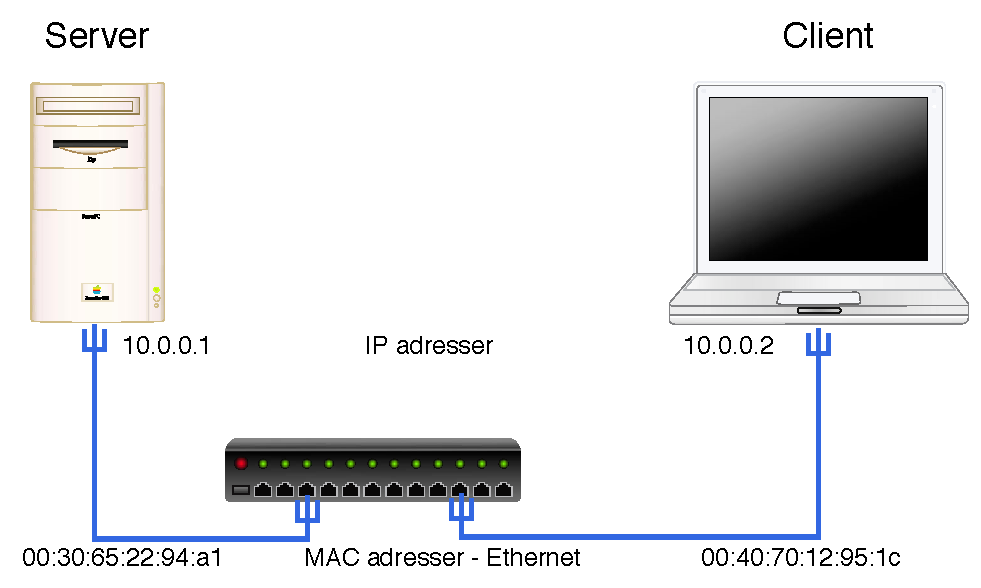
\includegraphics[width=18cm]{images/arp-basic.pdf}}  
\end{center}

%server 00:30:65:22:94:a1\\
%client 00:40:70:12:95:1c\\
%hacker 00:02:03:04:05:06\\

\slide{ARP request and reply}
\begin{list1}
\item {\bfseries ping 10.0.0.2} from server
\item ARP Address Resolution Protocol request/reply:
  \begin{list2}
  \item ARP request broadcasted on layer 2 - Who has 10.0.0.2 Tell 10.0.0.1
  \item ARP reply (from 10.0.0.2) 10.0.0.2 is at 00:40:70:12:95:1c
  \end{list2}
\item IP ICMP request/reply:
  \begin{list2}
    \item Echo (ping) request from 10.0.0.1 to 10.0.0.2
\item Echo (ping) reply from 10.0.0.2 to 10.0.0.1
\item ...
  \end{list2}
\item ARP is performed on Ethernet before IP can be transmitted
\end{list1}


\slide{ IPv6 neighbor discovery protocol (NDP)}

\hlkimage{20cm}{ipv6-arp-ndp.pdf}

\begin{list1}
\item ARP er v�k
\item NDP erstatter og udvider ARP, Sammenlign \verb+arp -an+ med \verb+ndp -an+
\item Til dels erstatter ICMPv6 s�ledes DHCP i IPv6, DHCPv6 findes dog
\item {\bf NB: bem�rk at dette har stor betydning for firewallregler!}
\item RFC4861 Neighbor Discovery for IP version 6 (IPv6)
\end{list1}

\slide{ARP vs NDP}

\begin{alltt}
\small
hlk@bigfoot:basic-ipv6-new$ arp -an        
? (10.0.42.1) at{\bf 0:0:24:c8:b2:4c} on en1 [ethernet]
? (10.0.42.2) at 0:c0:b7:6c:19:b on en1 [ethernet]

hlk@bigfoot:basic-ipv6-new$ ndp -an        
Neighbor                      Linklayer Address  Netif Expire    St Flgs Prbs
::1                           (incomplete)         lo0 permanent R      
2001:16d8:ffd2:cf0f:21c:b3ff:fec4:e1b6 0:1c:b3:c4:e1:b6 en1 permanent R      
fe80::1%lo0                   (incomplete)         lo0 permanent R      
fe80::200:24ff:fec8:b24c%en1 {\bf 0:0:24:c8:b2:4c}      en1 8h54m51s  S  R   
fe80::21c:b3ff:fec4:e1b6%en1  0:1c:b3:c4:e1:b6     en1 permanent R      
\end{alltt}

\slide{IPv6 firewalls }

\begin{alltt}\small
# Simple stateful network firewall rules for IPv6 
# using IPv4 file for input and inspiration from
# http://www.ipv6style.jp/en/building/20040526/2.shtml
# input from 
        $fwcmd6 -f flush
        $fwcmd6 add allow all from any to any via lo0
# Allow ICMPv6 destination unreach
        $fwcmd6 add pass ipv6-icmp from any to any icmptypes 1
# Allow NS/NA/toobig (don't filter it out)
        $fwcmd6 add pass ipv6-icmp from any to any icmptypes 2  
# Allow timex Time exceeded 
        $fwcmd6 add pass ipv6-icmp from any to any icmptypes 3  
# Allow parameter problem
        $fwcmd6 add pass ipv6-icmp from any to any icmptypes 4  
# IPv6 ICMP - echo request (128) and echo reply (129)
        $fwcmd6 add pass ipv6-icmp from any to any icmptypes 128,129
# IPv6 ICMP - router solicitation (133) and router advertisement (134)
        $fwcmd6 add pass ipv6-icmp from any to any icmptypes 133,134
# IPv6 ICMP - neighbour discovery solicitation (135) and advertisement (136)
        $fwcmd6 add pass ipv6-icmp from any to any icmptypes 135,136
\end{alltt}

\slide{IPv6 firewalls, cont. allowing services}

\begin{alltt}\small
#       Allow all established connections to persist (setup required
#       for new connections).
        $fwcmd6 add allow tcp from any to any established
        $fwcmd6 add allow tcp from any to any out setup
# allow access to my webserver and ssh
#       $fwcmd6 add allow tcp from any to any 80,443  setup
        $fwcmd6 add allow tcp from any to any $ssh  setup

# allow access to X11 forwarding over ::1
        $fwcmd6 add allow tcp from any to ::1 6010  setup

#       Politely rejects AUTH requests (e.g. email and ftp)
        $fwcmd6 add reset tcp from any to any 113 

#       Deny everything else ipv6
        $fwcmd6 add 65435 deny log ipv6 from any to any

\end{alltt}

\slide{Getting connected}

\begin{list1}
\item Native IPv6 - available at some hosting providers in DK
\item Automatic tunnels 6to4, Teredo etc.
\begin{list2}
\item 6to4 benytter IPv4 infrastrukturen
\item Teredo sender IPv6 gennem IPv4/UDP pakker
\end{list2}
\item Configured tunnels and tunnelbrokers
\begin{list2}
\item \link{http://sixxs.net} IPv6 Deployment \& Tunnel Broker
\item \link{http://he.net} hurricane electric internet services
\end{list2}

\end{list1}

\slide{Allocating IPv6 addresses} 

\begin{list1}
\item You have plenty!
\item Providers will typically get /32
\item Providers will typically give you /48 or /56
\item Your /48 can be used for:
\begin{list2}
\item 65536 subnets
\item Each subnet has $2^{64}$ addresses
\end{list2}
\end{list1}


\slide{Danish resources - get involved}

\hlkimage{10cm}{taskforce-logo.jpg}

\centerline{ Danish IPv6 task force - unofficial
\link{http://www.ipv6tf.dk}}

\slide{Conclusion}

\begin{center}
\vskip 5mm
{\color{titlecolor}\LARGE \bf IPv6 is here already - use it}
\vskip 5mm


\link{http://www.ipv6actnow.org/}

\link{http://digitaliser.dk/group/374895}

\link{http://www.ipv6tf.dk}
\end{center}
\vskip 1cm 

\myquestionspage

\slide{VikingScan.org - free portscanning}

\hlkimage{18cm}{vikingscan.png}
%\vskip 1cm 
%\centerline{\link{http://www.vikingscan.org}}

\slide{Referencer: netv�rksb�ger}

\begin{list2}
\item Stevens, Comer, 
\item Network Warrior
\item TCP/IP bogen p� dansk
\item KAME b�gerne
\item O'Reilly generelt IPv6 Essentials og IPv6 Network Administration  
\item O'Reilly cookbooks: Cisco, BIND og Apache HTTPD
\item Cisco Press og website
\item Firewall b�ger, Radia Perlman: IPsec, 
\end{list2}

\slide{B�ger om IPv6}

\begin{list1}
\item \emph{IPv6 Network Administration}
af David Malone og Niall Richard Murphy
 - god til real-life admins, typisk
O'Reilly bog
\item \emph{IPv6 Essentials} af Silvia Hagen, O'Reilly 2nd edition (May 17, 2006)
	god reference om emnet
\item \emph{IPv6 Core Protocols Implementation}
af Qing Li, Tatuya Jinmei og Keiichi Shima
\item \emph{IPv6 Advanced Protocols Implementation}
af Qing Li, Jinmei Tatuya og Keiichi Shima
\item - flere andre
\end{list1}

\hlkprofiluk

\end{document}
